%----------------------------------------------------------------
%
%  File    :  survey-academic.tex
%
%  Author  :  Keith Andrews, IICM, TU Graz, Austria
% 
%  Created :  27 May 93
% 
%  Changed :  22 Oct 2012
% 
%----------------------------------------------------------------


\chapter{Recommendation}
\label{chap:Recommendation}
 

\section{Recommendation}

For responsive design and techniques you should employ on your 
tables, we suggest: Alternate Row Highlighting, Long Two Column, and Fixed Header. As well 
the developer i.e. designer show take consist different techniques to different screen size. For 
example like it is on Figure 1.1 the three different screen sizes. For the biggest one 
you define the height and weight of yout table to 100\% of container. For Tablets we recomand the 
fixed header, and for small screen size like mobile devices  we recommand the Long Two Column technique. 
This is done in order to cover all posible screen(container) sizes. As well to be much easier to find
wanted data in table, please use Alternate Row Highlighting. To take a look how each of this 
techniques is working take a look on previous chapters. How our recommentation table look like, 
you can see in following figure. 

\begin{figure}[H]
    \centering
  
    {%
    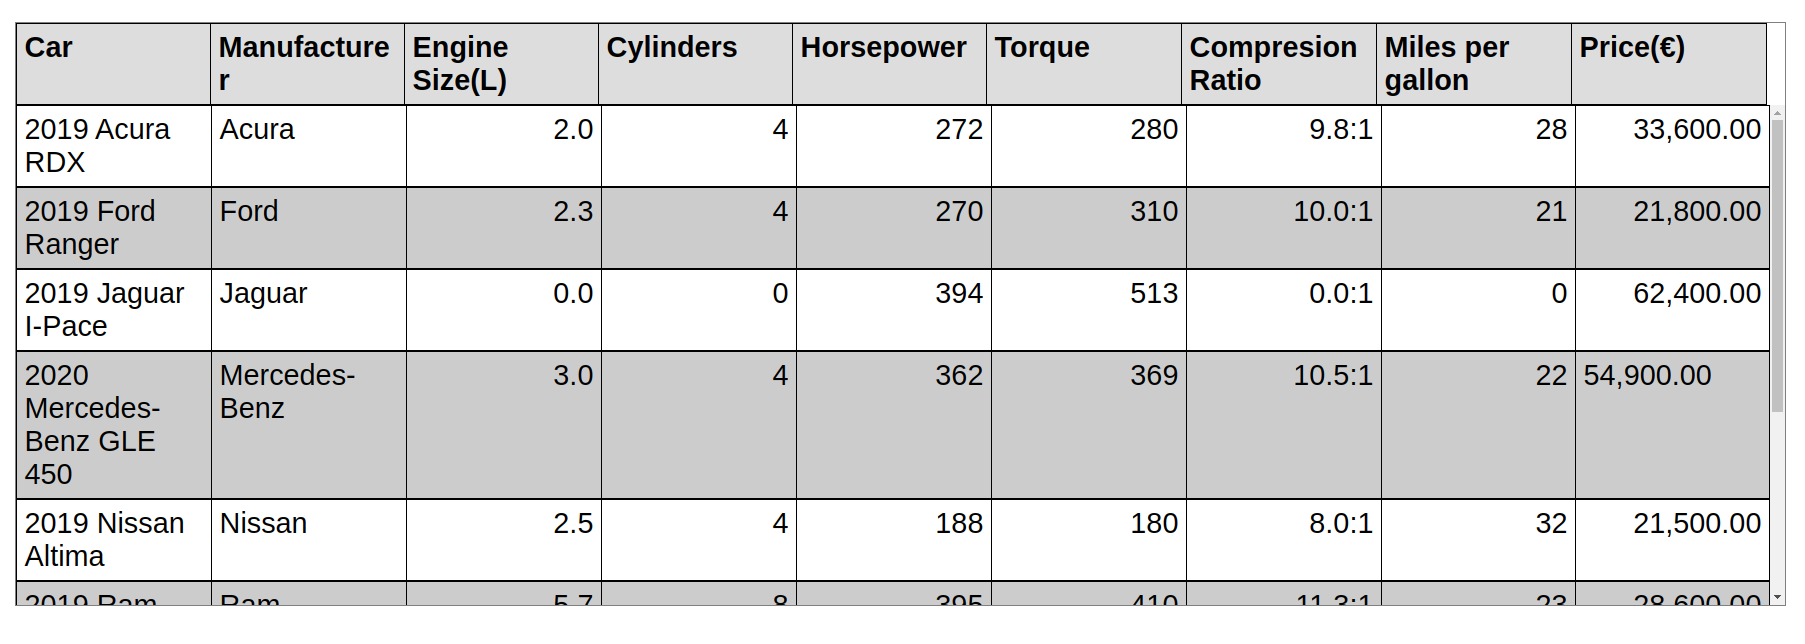
\includegraphics[width=1\linewidth]
    {recommendation.png}%
    \label{alig1}%
    }

    
    \caption[Recommendation Techniques]
    {
      
    \imgcredit{Screenshot taken by the author.}
    }
    \label{figWhol}
\end{figure}






